%%%%%%%%%%%%%%%%%%%%%%%%%%%%%%%%%%%%%%%%%%%%%%%%%%%%%%%%%%%%%%%%%%%%%%%%%%%%%%%
%%%%%%%%%%%%%%%%%%%%%%%%%%%%%%%%%%%%%%%%%%%%%%%%%%%%%%%%%%%%%%%%%%%%%%%%%%%%%%%
%                      PREAMBLE
%%%%%%%%%%%%%%%%%%%%%%%%%%%%%%%%%%%%%%%%%%%%%%%%%%%%%%%%%%%%%%%%%%%%%%%%%%%%%%%
%%%%%%%%%%%%%%%%%%%%%%%%%%%%%%%%%%%%%%%%%%%%%%%%%%%%%%%%%%%%%%%%%%%%%%%%%%%%%%%
\documentclass[11pt]{article}


\usepackage[T1]{fontenc}  % Better font encoding
\usepackage[utf8]{inputenc}

\usepackage{mathpazo}     % Palatino font with matching math fonts
\usepackage[french]{babel} % Use 'french' instead of 'français' for babel compatibility

\usepackage{graphicx}
\usepackage{tikz}
\usetikzlibrary{positioning}
\usepackage{subcaption}
\usepackage{amsmath}
\usepackage{mathtools}  % For \coloneqq
\usepackage{amssymb}
\usepackage{amsthm}  % For proof environment

\usepackage{bbm}  % For \mathbbm command
\usepackage[margin=2.5cm]{geometry}
\usepackage{float}

\setlength{\parindent}{0pt}

\title{\textbf{DEVOIR COURS IMAGE ARIA}}
\author{Abel Verley}
\date{}


\begin{document}

\maketitle

\textbf{Question 1 :}\\

On commence par définir un réseau LeNet et on l'entraine sur les données MNIST, comme dans le TP du cours, la fonction de perte utilisée étant l'entropie croisée. Le figure \ref{fig:loss_curve} ci-contre montre l'évolution de la fonction de perte au cours des 10 epochs d'entrainement du modèle, qui diminue comme voulu. 

\begin{figure}[H]
    \centering
    \begin{subfigure}[b]{0.48\textwidth}
        \centering
        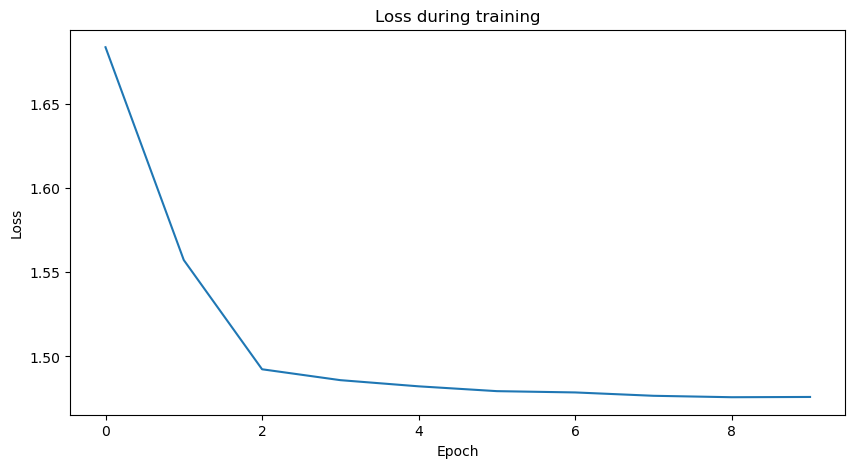
\includegraphics[width=\textwidth]{../plots/loss_curve.png}
        \caption{Évolution de la fonction de perte lors de l'entraînement.}
        \label{fig:loss_curve}
    \end{subfigure}
    \hfill
    \begin{subfigure}[b]{0.48\textwidth}
        \centering
        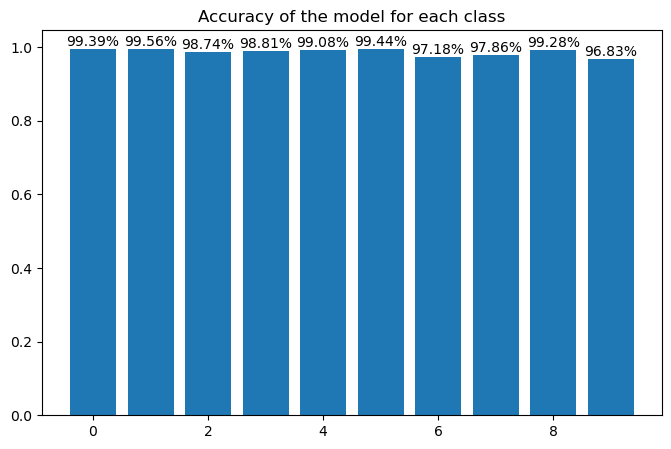
\includegraphics[width=\textwidth]{../plots/accuracy_class_LENET.png}
        \caption{Évolution de la précision lors de l'entraînement.}
        \label{fig:accuracy_curve}
    \end{subfigure}
    \caption{Courbes de perte et de précision lors de l'entraînement du modèle LeNet sur MNIST.}
    \label{fig:training_curves}
\end{figure}

Après entraînement, notre modèle performe avec un précision de 98,62\% sur le jeu de données test, et le détail de la précision par classes d'image est donnée dans la figure \ref{fig:accuracy_curve} ci-dessus : les 9, les 6 et les 7 sont les moins bien classifiés, là où les 1 sont les mieux classifiés. \\

On implémente ensuite la méthode Fast Gradient Sign Attack (FGSA) où une image est perturbée dans la direction du gradient de la fonction de perte, de sorte à tromper le modèle :
\begin{equation}
    x_{adv} = x + \varepsilon \cdot sign(\nabla \mathcal{L}(x,y)) 
\end{equation} 

Pour une valeur de $\varepsilon = 0.3$, l'attaque à un taux de succès de 39.3\% sur le jeu de données test. La figure \ref{fig:fgsm_examples} montre des exemples de l'effet de l'attaque et on voit que le 1 est classifié comme 4 dans sa version bruitée. 

\begin{figure}[H]
    \centering
    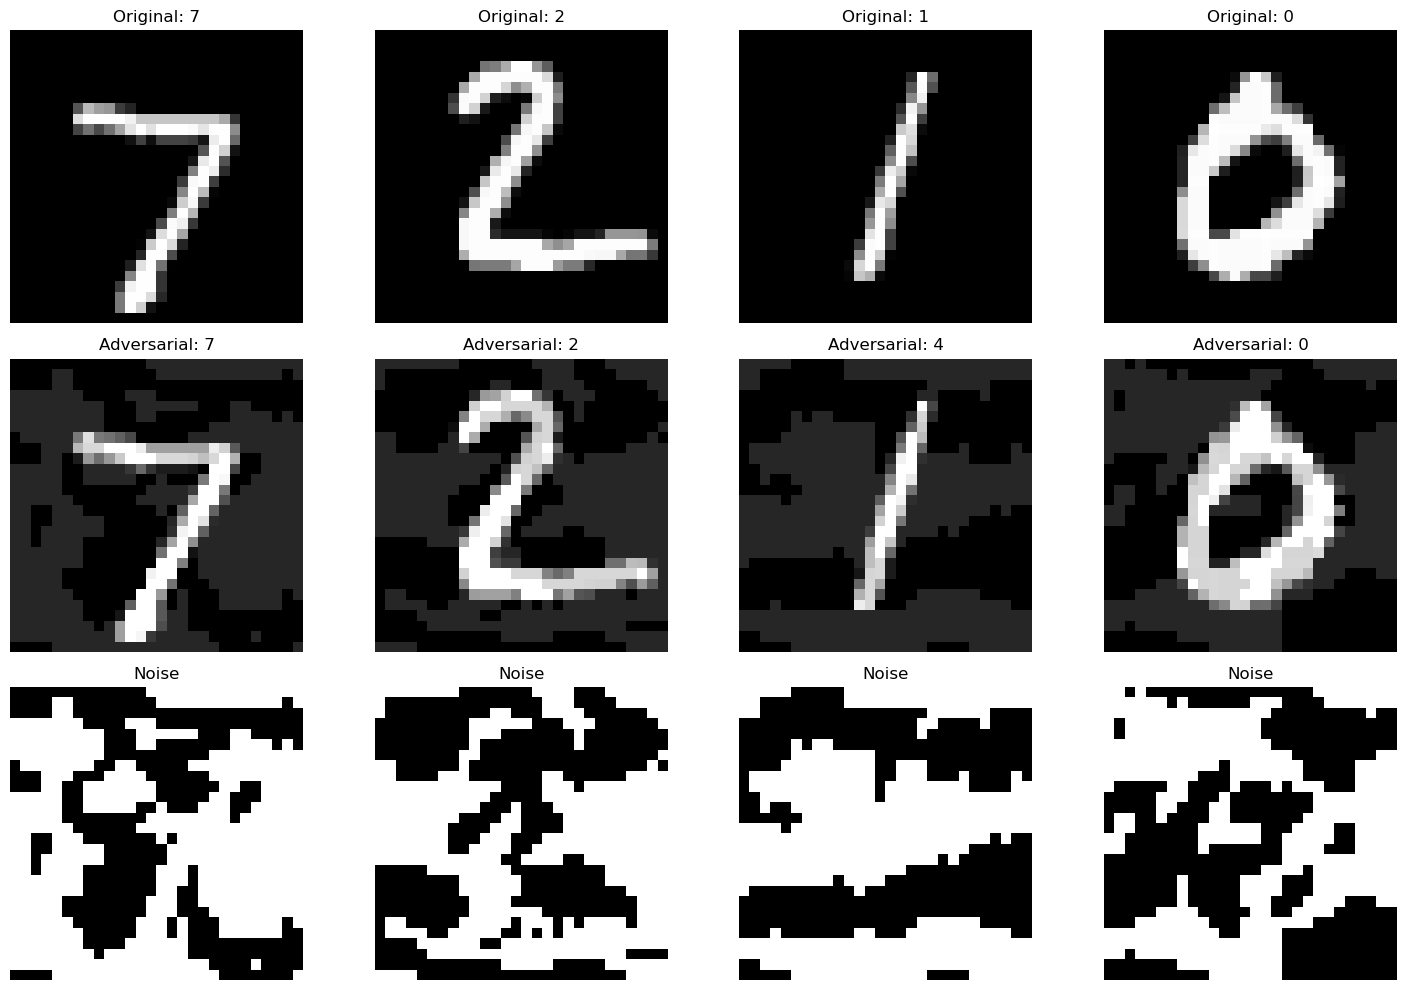
\includegraphics[width=0.6\textwidth]{../plots/adversarial_examples.png}
    \caption{Exemples d'images MNIST originales et prédiction(ligne du haut) et leurs versions adversariales générées avec FGSM et $\varepsilon = 0.3$ et prédiction(ligne du milieu) et bruit (ligne du bas). }
    \label{fig:fgsm_examples}
\end{figure}


\textbf{Question 2 : } \\

Comme le montre la figure, augmenter le paramètre $\varepsilon$ a une influence directe sur le rendu visuel de l'image, et rend l'attaque plus facilement détectable. 

\begin{figure}[H]
    \centering
    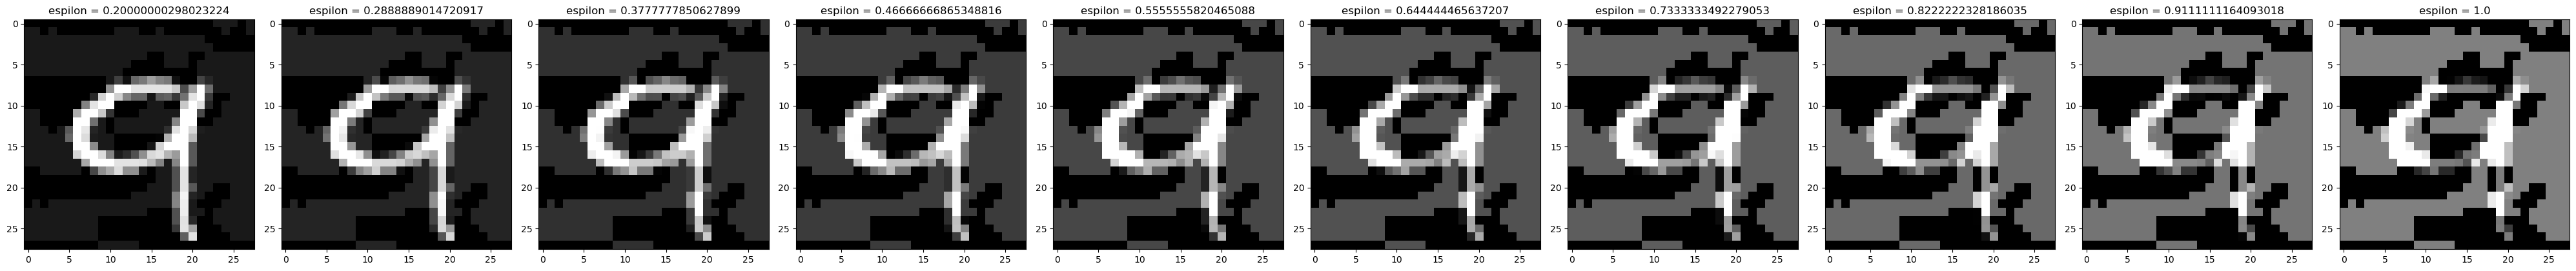
\includegraphics[width=\textwidth]{../plots/epsilon_influence.png}
    \caption{Effet de différentes valeurs de $\varepsilon$ sur l'apparence des images MNIST attaquées par FGSA}
    \label{fig:epsilon_grid}
\end{figure}

On s'intéresse aussi au taux de succès de l'attaque en fonction de la valeur de $\varepsilon$ et en fonction de la classe. On obtient alors les courbes de la figure \ref{fig:fsga_success} suivante. Comme on pourrait s'y attendre, plus $\varepsilon$ augmente, plus le taux de succès de FGSA est élevé. On remarque aussi que toutes les classes ne réagissent pas de la même manière à l'attaque : ici, la classe 1 se retrouve très vite impactée à l'inverse de la classe 3. Cependant, après avoir fait plusieur essais, il semblerait que l'ordre des classes les plus impactée varie beaucoup selon les testes (dû à l'aléatoire de l'initialisation du modèle et à la stochasticité de l'algorithme ADAM).

\begin{figure}[H]
    \centering
    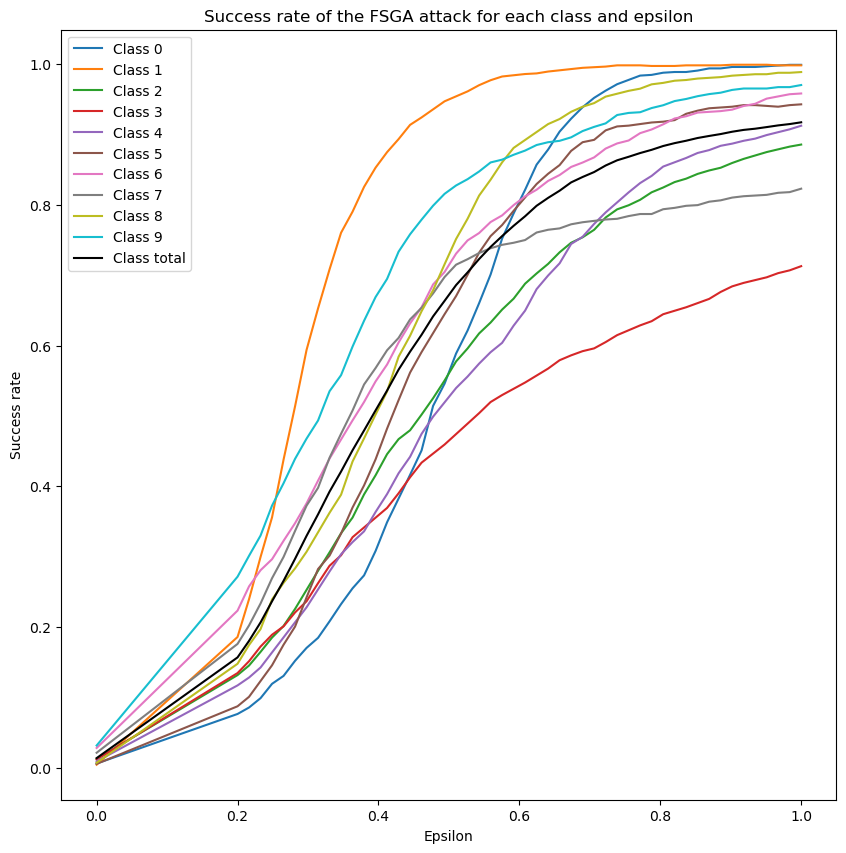
\includegraphics[width=0.5\textwidth]{../plots/success_FSGA.png}
    \caption{Evolution du taux de success de FGSA en fonction de la valeur $\varepsilon$ et en fonction de la classe}
    \label{fig:fsga_success}
\end{figure}

\textbf{Question 3 :}\\

On compare maintenant la FGSA avec l'ajouts d'un bruit gaussien de variance $\varepsilon$ :  

\begin{figure}[H]
    \centering
    \begin{subfigure}[b]{0.48\textwidth}
        \centering
        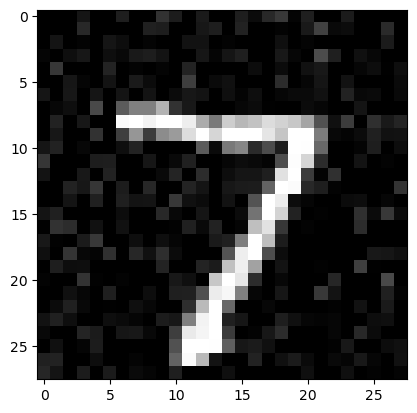
\includegraphics[width=\textwidth]{../plots/white_noise_example.png}
        \caption{Perturbation d'une image MNIST par ajôut de bruit blanc ($\varepsilon = 0.3$).}
        \label{fig:white_noise}
    \end{subfigure}
    \hfill
    \begin{subfigure}[b]{0.48\textwidth}
        \centering
        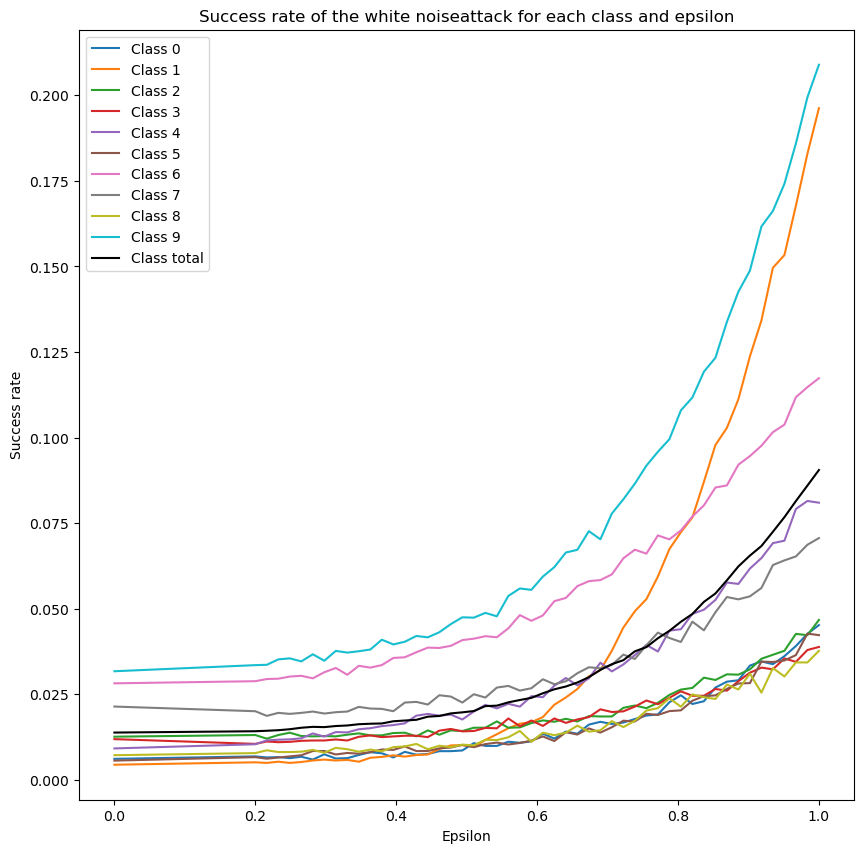
\includegraphics[width=\textwidth]{../plots/white_noise_success.png}
        \caption{Performances de l'attaque par bruit gaussien}
        \label{fig:white_noise_success}
    \end{subfigure}
    \caption{Illustration de l'attaque par ajout de bruit gaussien}
    \label{fig:fgsm_vs_gaussian}
\end{figure}

On voit dans la figure \ref{fig:white_noise} que l'ajout de bruit blanc est beaucoup plus dispersé sur l'image que celui de la FGSA. La figure \ref{fig:white_noise_success} que le modèle LeNet entraîné et nettement plus résistant au bruit blanc qu'à la FGSA. Pour une variance de 1, le taux de succès de l'attaque est seulement de 0.1 et classe la plus vulnérable est le 9 qui atteint un taux de succès de 0.2.\\


\textbf{Question 4 :} \\

On peut conclure des résultats précédents que dans un cas d'application réel, les classifieurs comme LeNet vont être très résistants au bruit naturel qui a une nature plutôt gaussienne. Cela veut aussi dire qu'il faut utiliser des méthodes plus sophistiquées, telles que FGSA, pour tromper un classifieur. Mais notons que la FGSA est difficile à mettre en place en pratique car elle requière d'avoir accès au modèle pour calculer le gradient de la fonction de perte. \\

\textbf{Question 5 :}\\

Finalement pour cette question on se propose de réentrainer le modèle sur une base de donnée contenant des exemples adversariaux pour différentes valeurs de $\varepsilon$. Plus précisément, on prend 50 valeurs de $\varepsilon$ réparties linéairement entre 0.2 et 1, puis la nouvelle base de données d'entrainement contient en plus 50 versions de la précédente où chaque image est perturbée par FGSA avec le gradient d'un modèle entraîné. On entraine alors un nouveau modèle LeNet sur cette base de données augmentée que l'on teste sur le jeu de données test, lui même perturbé par FGSA. On obtient la figure \ref{fig:adversarial_training} suivante qui montre que le modèle est bien plus résistant à l'attaque et que l'attaque échoue dans plus de 95\% des cas. On remarque une performance optimal de la stratégie d'appretissage adversarial autour de $\varepsilon=0.4$. Néanmoins, une contrepartie est que, puisqu'une large marjorité du jeu d'entrainement est bruité, le modèle classifie mieux certaines images bruitées que d'autres non bruitées.


\begin{figure}[H]
    \centering
    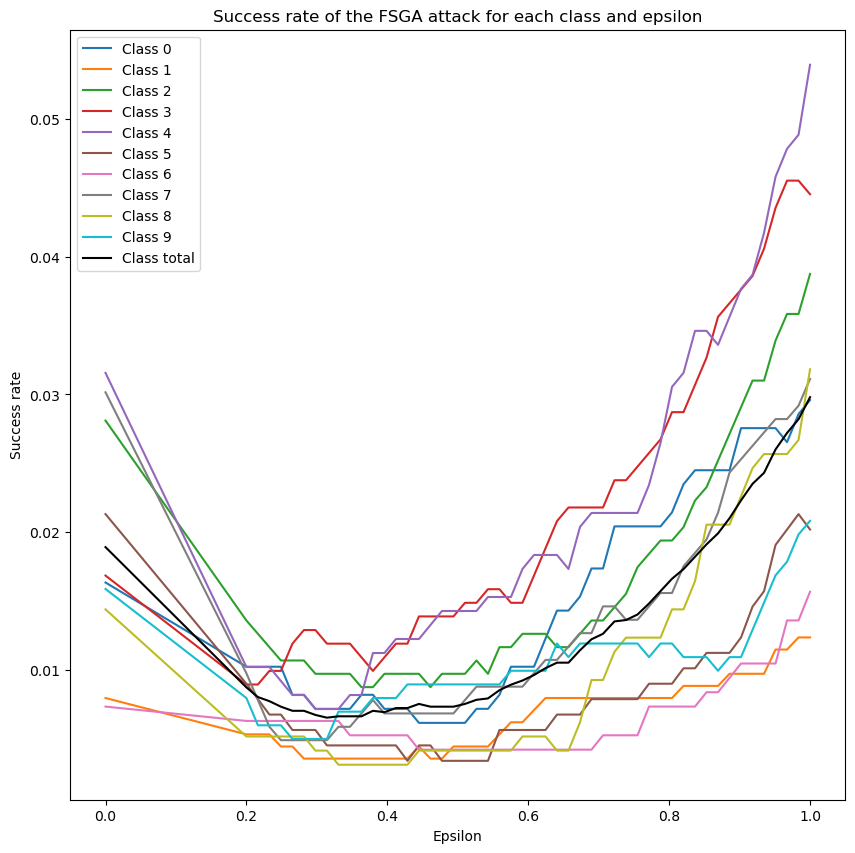
\includegraphics[width=0.5\textwidth]{../plots/adversarial_training.png}
    \caption{Performance du modèle après entraînement adversarial : taux de succès de FGSA en fonction de $\varepsilon$ .}
    \label{fig:adversarial_training}
\end{figure}

\end{document}